
\begin{figure}
    \centering
    \begin{subfigure}[b]{0.45\textwidth}
        \centering
        
\includegraphics[scale=2.0]{resources/mnist4.jpg}
        \caption{Four digits without noise.
        %, size $112 \times 28$.
        }
        \label{fig:mnist4}
    \end{subfigure}%
    \begin{subfigure}[b]{0.45\textwidth}
        \centering
        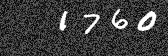
\includegraphics[scale=2.0]{resources/random_pad.jpg}
        \caption{Random position and dot noise.
        %Four digits with noise.
        %at a random position inside a box of $168 \times 56$ with dot noise.
        }
        \label{fig:mnist_random_pad}
    \end{subfigure}
    \caption{Two types of generated synthetic data from MNIST. The relative size between the two examples is preserved.}
\end{figure}